
\chapter{2D simulations for a simplified upper-core model}

\label{chap:3}
\vspace*{-12mm}
{\footnotesize \sl
Section \ref{sec:2DGRF} of this chapter has been published as an article in an international journal, under the reference: Masaru Nagaso, Joseph Moysan, Sa\"{\i}d Benjeddou, Nicolas
Massacret, Marie-Aude Ploix, Dimitri Komatitsch and Christian Lhuillier, Ultrasonic thermometry simulation in a random fluctuating medium: Evidence of the
acoustic signature of a one-percent temperature difference, Ultrasonics, vol. 68, p. 61-70, doi: 10.1016/j.ultras.2016.02.011 (2016).}

\vspace*{+2mm}
    In this chapter, we will first perform a comparative study between several Finite Difference in the Time Domain (FDTD) numerical schemes and a Spectral-Element Method (SEM)
to simulate ultrasonic wave propagation in the core of a sodium reactor. From these results, we will show that
the SEM scheme has high computational stability and efficiency for our modeling purposes.
    After the experimental study of the accuracy properties of these two numerical simulation techniques,
we will perform a 2D simulation study with a Gaussian random field to introduce heterogeneity in the propagation medium.
We will analyze the effects of stochastically-generated
temperature fluctuation fields on 2D acoustic wave propagation, and the feasibility and accuracy of ultrasonic thermometry at the upper-core region of a sodium-cooled fast reactor.

    \section{Validation of the SPECFEM numerical code for our problem, and comparison with other numerical schemes}
    \label{sec:UPSILON}

\vspace*{-3mm}
        In order to gain good knowledge about features of numerical modeling methods for ultrasonic wave propagation in a sodium reactor core, let us compare the acoustic fields
calculated based on several types of full waveform modeling methods. We use the configuration of an experiment performed at CEA Cadarache and called UPSILON in order to see the effect of temperature heterogeneity on the
accuracy and stability of the numerical simulations. For these purpose, we used the numerical code SPECFEM for the SEM calculations and SEISMIC\_CPML for the FDTD
calculations.

    \subsection{SEISMIC\_CPML}

        SEISMIC\_CPML is a software package that was developed mostly by Dimitri Komatitsch and Roland Martin at CNRS. As SPECFEM,
SEISMIC\_CPML is an open-source code distributed by the Computational Infrastructure for Geodynamics (CIG, \url{http://geodynamics.org/cig/software/seismic_cpml}).
        It can solve two/three-dimensional isotropic/anisotropic acoustic/elastic and viscoelastic/poroelastic wave equation based
on finite differences in the time domain. Convolutional perfectly matched absorbing layers \citep{KoMa07} are also implemented to mimic infinite or semi-infinite propagation media.
More details about SEISMIC\_CPML can be found at \url{http://komatitsch.free.fr/README_seismic_cpml.html}
For our comparisons, we improved this code by increasing the order of spatial discretization, i.e., we increased the number of grid points that are used for the calculations
of derivatives at a given grid point. We also modified the 2D version of the code
to support parallel computing based on MPI (the 3D version of the code already had such parallel support based on MPI, but the 2D pressure version
did not). Thanks to these two improvements, we managed to simulate wave propagation for
high-frequency (\SI{2.25}{\mega\hertz}) acoustic emission, with low computational error and high stability and with significantly shorter computational time.

    \subsection{Simulation for the UPSILON experiment}

        UPSILON is an experiment that was designed to observe how an acoustic wave is affected by thermal heterogeneity in silicon oil.
This experiment has initially performed by Nicolas Massacret in his Ph.D. study at CEA/LIET \citep{Massacret2014Etudedunemethode}.
The heterogeneity of the temperature field in silicon oil is
generated by heating wires, and changes in an acoustic wave front may be observed from recorded acoustic signals using a Schlieren optical system.
Table \ref{table:upsilon_tools} shows the names and specifications of equipments used in this experiment.
        We therefore decided to model the UPSILON configuration in our acoustic wave propagation numerical simulations. The model geometry is shown in Figure \ref{fig:upsilon_conf}.
        We computed wave propagation for two states of the propagation medium, one with a homogeneous medium and the other with the same geometrical configuration but
with a heterogeneous medium. The sound velocity field is calculated based on
\begin{align} \label{eq:2_11_1}
    C_p = 1056.60 - 2.72 T_{Celcius} \, .
\end{align}

        \begin{figure}[htbp]
                \centerline{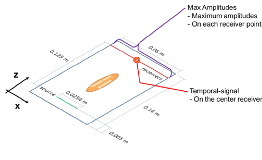
\includegraphics[width=12cm]{upsilon_conf_v2.pdf}}
            \slantedcaption{Configuration of the models for our simulations. The UPSILON experiment is modeled in two dimensions. The green line is the
source line that emits a quasi-plane wave. The elliptical part in orange is the heated area.}
            \label{fig:upsilon_conf}
        \end{figure}

The shape of the heated area and medium
temperature is defined by Equation \ref{eq:2_11} in all heterogeneous simulations.
The density of silicon oil was calculated based on the equation of sound speed for a fluid $c=\sqrt{K/\rho}$
where $c$ is sound speed, $K$ is the bulk modulus, and $\rho$ is density.
$K$ was calculated from the known density value of silicon oil from its specification sheet: \SI{970}{\kilo\gram\per\cubic\metre}.
An acoustic emission surface is modeled as a line source (represented by the green line in Figure
\ref{fig:upsilon_conf}) composed of many individual point sources placed on a straight line. A Ricker time wavelet (i.e., the second derivative of a Gaussian)
is emitted from all these source points, and a Hamming window
function is applied to the amplitude of each emission depending on the distance of that source to the central point of the line source in order to emit a
quasi-plane wave:
        \begin{align} \label{eq:2_11}
            T(x,z)=20.00+8.00e^{-5.00*10^4(x-0.03)}\frac{1}{1+e^{400(z-0.08)}}\frac{1}{1+e^{400(-z+0.08)}}.
        \end{align}

        \begin{table}
            \slantedcaption{Names and specifications of the different equipments used in the UPSILON experiment by \cite{Massacret2014Etudedunemethode}.}
\vspace{5truemm}
            \makebox[1 \textwidth][c]{
            \resizebox{1. \textwidth}{!}{
            \begin{tabularx}{\textwidth}{llll}
                \hline
                Name & Manufacturer & Product & Others \\ \hline
                Silicon oil & Carl Roth Silicon Oil & M 10,000 cSt & \parbox[t]{4cm}{density at 20$\degree$:\\\num{970} - \num{980} \si{kg/m^3}} \\
                \parbox[t]{2cm}{Acoustic probe\\(emitter)}  & Olympus Panametrics & \parbox[t]{4cm}{Standard Contact Video Scan,\\V104-RB} &
\parbox[t]{4cm}{Mono-element,\\frequency 2.25 MHz,\\surface diameter \SI{3.175}{\centi\meter}} \\
                \parbox[t]{2cm}{needle\\hydrophone\\(receiver)} & No data & No data & \parbox[t]{4cm}{bandwidth 1-10 MHz}\\ \hline
            \end{tabularx}
            }
            }
            \label{table:upsilon_tools}
        \end{table}

            Figure \ref{fig:upsilon_geo} shows the experimental configuration of UPSILON. The formulation for sound velocity \ref{eq:2_11_1} is an empirical formula
that was experimentally established by \cite{Massacret2014Etudedunemethode}. The ultrasonic emitter at \SI{2.25}{\mega\hertz} has a diameter of 1 inch (i.e. \SI{2.54}{\centi\meter}),
and the profile of the acoustic field is measured using a quarter-inch plane receiver at \SI{2.25}{\mega\hertz} to obtain a fine measurement.
            Thermocouples are used to measure temperature in the area of interest, and a polynomial variation is used to describe the distribution of temperature.
This polynomial expression was then simplified using the symmetric formula of Equation~\ref{eq:2_11} in order to make simulations easier to perform.
            This experiment was efficient to illustrate the phenomena that were looked for: deviation of ultrasounds by temperature gradients, and wave speed variations.
To our knowledge it was the first demonstration that ultrasonic measurement techniques are accurate enough to detect thermal-hydraulic effects on wave propagation.
The originality of this experiment was to create a localized and stable temperature gradient thanks to the thermal silicon oil properties.

    \begin{figure}[htbp]
            \centerline{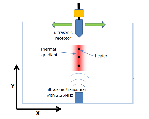
\includegraphics[width=12cm]{upsilon_geo.pdf}}
            \slantedcaption{Experimental configuration of UPSILON, taken from \cite{Massacret2014Etudedunemethode}.}
        \label{fig:upsilon_geo}
    \end{figure}


    \subsection{Results of the comparisons between the different numerical schemes}

We compared results obtained with the SEM technique with those obtained based on the standard FDTD, Optimized-FDTD, and NSFDTD schemes presented in the previous chapter.
        First, we performed convergence tests for both homogeneous and heterogeneous cases of all schemes by changing the number of grid points per
wavelength in the case of FDTD, or the number of spectral elements per wavelength in the case of the SEM. In the FDTD tests, 10, 20, 25, 30, 35, 40 points per wavelength were tested.

Excellent convergence for this very sensitive (and thus very difficult) test was obtained with 40 points per wavelength
for Optimized-FDTD and NSFDTD, but second/fourth order FDTD could not achieve convergence even with
40 nodes per wavelength in the homogeneous case.
For the SEM, we tested 1, 2, 4, 6 elements per wavelength and achieved excellent convergence with 4 or 6 elements per wavelength.
        We compared all schemes based on two criteria: maximum amplitude values recorded at each receiver point on the receiver line indicated as the orange
line in Figure \ref{fig:upsilon_conf}, and the single signal recorded at the center of the receiver line.

        Figure \ref{fig:upsilon_res1} of upper row shows the results of comparison between all schemes for the homogeneous simulation, and Figure \ref{fig:upsilon_res1} of lower row shows the
results for the heterogeneous case. In the homogeneous results, SEM (SPECFEM2D), optimized-FDTD and NSFDTD converge to extremely similar results,
while the signals of second/fourth-order FDTD still exhibit dispersion of the signal peaks i.e. they have not yet fully converged.
Because this configuration of acoustic emission involves very high frequency
waves, it requires very high resolution for the spatial discretization, and this is why second/fourth-order spatial orders based on classical schemes
are not sufficient for this numerical experiment, considering also the very large total number of time steps involved, i.e. the cumulative numerical dispersion involved.

On the other hand, it is clear that the SEM reaches convergence with a smaller
number of grid points than the other schemes, which is directly linked to the reduction of the required amount of computational resources (in the SEM,
spectral elements with fourth-order polynomial basis functions have 4 computation nodes for each element, thus 6 elements per wavelength is approximately equivalent to 24 grid points
per wavelength). This means that the required number of grid points for convergence of the SEM calculation is 24 (nodes for SEM) / 40 (nodes for FDTD) \string^ 2 (the number of spatial dimensions) * 100 (\%) = \SI{36}{\percent} of the number of nodes required for FDTD in the two-dimensional case;
in the three-dimensional case, only 24/40 \string^ 3 (number of spatial dimensions) * 100(\%) = \SI{21.6}{\percent} of the nodes required for 3D FDTD are necessary for convergence of the 3D SEM calculation.

\noindent
        In the heterogeneous results in Figure \ref{fig:upsilon_res1} at the lower row, the curve of second-order FDTD is not shown because its calculation did not converge.
Again, the fourth-order FDTD results exhibit numerical errors appearing for instance as dispersion of the peaks. Each temporal signal has two peaks
while the homogeneous case has only one peak. This is because the direct wave which passed through the center of the heated medium was significantly slowed down.
Instead, the wave that traveled through colder regions of the medium arrives at the central receiver faster by going around the hot spot, and the slowed direct
wave arrives later, which explains why the second peak has a larger value than the first.
        The curves obtained based on all the other schemes (on the right-hand side of the figure) are all very close,
however we still find some differences between the curves of the max amplitude (on the left-hand side of the figure),
which comes from the fact that the maximum amplitude curve is very sensitive to the change of shape of the wave front.

        We calculated the correlation coefficients between SEM and other method for homogeneous and heterogeneous case. To do so, we used the temporal signals recorded at the
center of the receiver line. The results are shown in Table \ref{table:upsilon_res3}. It is clear that for both the homogeneous and heterogeneous cases that NSFDTD
and optimized-FDTD have higher correlation coefficients than the two more classical but less accurate methods.

        \begin{figure}[htbp]
                \centerline{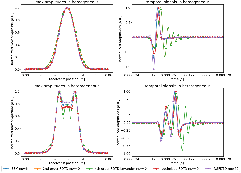
\includegraphics[width=\textwidth]{upsilon_res.pdf}}
            \slantedcaption{Comparison between SEM, 2nd/4th-order FDTD, Optimized-FDTD, NSFDTD in the homogeneous case (upper row) and in the heterogeneous case (lower row).}
            \label{fig:upsilon_res1}
        \end{figure}

        \begin{table}
            \centering
            \slantedcaption{Correlation coefficients between SPECFEM and different FDTD schemes. The temporal signal of each scheme at the center of the receiver
line is used for this comparison.}
\vspace{5truemm}
            \begin{tabular}{lll}
                \toprule
                Computation scheme & Homogeneous & Heterogeneous \\ \midrule
                Second-order FDTD     & \num{4.22143e-1} & Did not converge \\
                Fourth-order FDTD     & \num{4.22105e-1} & \num{4.57660e-1}   \\
                NSFDTD             & \num{9.53819e-1} & \num{9.54614e-1}   \\
                Optimized-FDTD     & \num{9.54240e-1} & \num{9.52261e-1}   \\ \bottomrule
            \end{tabular}
            \label{table:upsilon_res3}
        \end{table}

In future work, Massacret's Upsilon experiment should be improved by using a 2D matrix transducer in order to be able to perform a 3D comparison between experiments and modeling.
This discussion of such future work will be continued in the Conclusions and perspective chapter (\autoref{chap:5}).
We can conclude that the SEM has advantages not only because of its capacity to model curved geometrical surfaces thanks to
the finite-element discretization scheme involved, but also thanks to its capacity to achieve convergence with smaller computational resources.
Let us mention that in the calculations based on SPECFEM, we used a very accurate Low-dissipation and low-dispersion Runge-Kutta (LDDRK) time scheme \citep{Berland2006Lowdissipationand}
for time marching, while for FDTDs we used a standard Newmark scheme \citep{Hug87}.
This difference thus favors the SEM results when a large number of time steps is involved.

\section{Ultrasonic thermometry simulation in a random fluctuating medium: Evidence of the acoustic signature of a one-percent temperature difference}
\label{sec:2DGRF}

Let us now study the development potential of ultrasonic thermometry in a liquid fluctuating sodium environment similar to that present in a Sodium-cooled Fast
Reactor, and thus investigate if and how ultrasonic thermometry could be used to monitor the sodium flow at the outlet of the reactor core. In particular we
study if small temperature variations in the sodium flow of e.g. about \SI{1}{\percent} of the sodium temperature, i.e., about 5\textdegree{}C, can have a
reliably-measurable acoustic signature. Since to our knowledge no experimental setups are available for such a study, and considering the practical
difficulties of experimentation in sodium, we resort to a numerical technique for full wave propagation called the spectral-element method, which is a highly
accurate finite-element method owing to the high-degree basis functions it uses. We obtain clear time-of-flight variations in the case of a small temperature
difference of one percent in the case of a static temperature gradient as well as in the presence of a random fluctuation of the temperature field in the
turbulent flow. The numerical simulations underline the potential of ultrasonic thermometry in such a context.

    \subsection{Positioning of the problem}

        Our work aims at studying potential improvements upon temperature sensors currently used for sodium temperature measurements, such as thermocouples, by resorting to
ultrasonic thermometry. Ultrasonic thermometry can be implemented based on several approaches. A first one consists of using an ultrasonic thermometer: by
sending an ultrasonic pulse through a thin rod with acoustic discontinuities such as notches or sudden diameter changes, and measuring the time between the
initial pulse and the reflections of that pulse, the rod is segmented into a multi-point temperature sensor \parencite{Daw2002Ultrasonicthermometryfor}. For
our study however, the starting point regarding thermometry for in-service temperature measurement at the outlet of the core is a second approach described in
a 1985 British patent registered by A. McKnight et al. entitled "Remote temperature measurement" \parencite{McKnight1987Remotetemperaturemeasurement}. The
main idea in that patent is to use an ultrasonic beam that impinges on the two diametrically opposite edges of a subassembly separated by a known distance.
Measuring the time interval between the two echoes (and knowing the relation between celerity and temperature) then allows one to deduce the mean temperature
of the liquid sodium between these two points.

        However, since several parameters can influence the time-of-flight measurement, several challenging issues need to be addressed in order for such a
technique to be usable in practice. The liquid sodium exiting the core of a nuclear reactor is a turbulent flow with thermal heterogeneities, and local flow
variations can thus influence wave propagation. The shape of the reflected echoes, which depends on the fuel assembly geometry, can also be of importance and
should be taken into account in the signal processing method used. In some particular cases, the proportion of gas micro-bubbles can also vary and modify the
relation between celerity and temperature. Recent work has specifically focused on these aspects of wave propagation in a turbulent medium
\parencite{Massacret2014Modellingofultrasonic} as well as evaluation of gas proportion in an SFR \parencite{Cavaro2011Microbubblecloudcharacterization}.

        In this study our goal is to study the development potential of ultrasonic thermometry in liquid sodium and thus to investigate if and how ultrasonic
thermometry could be used to monitor the outlet of a sodium reactor core. In particular we want to see if small temperature variations (of e.g. about
\SI{1}{\percent} of the sodium temperature, i.e., about 5\textdegree{}C) in the sodium flow could have a reliably-measurable acoustic signature. The gas
proportion is considered as constant in our study and flow rate is also neglected. Since to our knowledge no operating experimental setups would allow us to
obtain a precise description of the fluctuating medium, and considering the practical difficulties related to experimentation in sodium, we will turn to
highly-accurate numerical modeling based on a full wave modeling technique.

        One of the difficulties in order to get a good model is to define what a liquid-sodium fluctuating medium can be. Its temperature and flow velocity
field fluctuate by the interaction of a flow and the core structure composed of various assemblies, and they also fluctuate due to the thermo-dynamical
equilibrium of the medium.
To the best of our knowledge, no Computational Fluid Dynamics code can accurately generate such media at reasonable cost at a scale
compatible with the ultrasonic scale that we want to target. We will thus turn to physical modeling to generate the fluctuating medium.
In general, physical characteristics of a heterogeneous liquid medium fluctuate spatially and temporally, depending on its nature and on the environment.
Such a heterogeneity is quite complex to model in a deterministic way because of many uncontrolled factors and thus it is common to model them based on a stochastic process.
This issue has been addressed in the literature regarding modeling of heterogeneous liquid sodium in the context of wave propagation simulation.

        In order to verify the possibility of measuring a small temperature variation in such an environment, which is the main goal of our study, it is
necessary to consider the effect of temperature fluctuations caused by turbulent flow. For this purpose, we regard the temperature field as a combination of a
static temperature distribution, which is to be measured, and a fluctuation part. Considering that fluctuating part, we resort to the Gaussian random field
method, which is a random field generator based on a spectral method introduced by \textcite{Shinozuka1972Digitalsimulationof}.

        The section will be structured as follows: In \autoref{ssec:2dgrf_the} we will describe the thermometry concept at the outlet of the fuel assembly. In \autoref{ssec:2dgrf_num} we will describe the configurations defined for our simulations and the definition of the temperature fields. We will then discuss the results and show that our 2D numerical simulations underline the potential of ultrasonic thermometry in \autoref{ssec:2dgrf_res}.

    \subsection{Thermometry at the outlet of nuclear fuel assemblies} \label{ssec:2dgrf_the}
        Current setups for thermal instrumentation above a reactor core consist of hundreds of thermocouples assembled in thermo-wells, one above each fuel
assembly that needs to be monitored. However, as indicated above, there is a need for developing more efficient instrumentation for the next generation of
nuclear reactors. One important issue to address is the ability to perform faster measurements, as the expected response time of the complete temperature
instrumentation in these future reactors is 0.1 s or even less instead of at best about 1 s with sheathed thermocouples. Another interest for the ultrasonic
method is that it is less sensitive to sodium jet bending than thermocouples. Additional improvements could consist of reducing the number of electrical wires
located above the reactor core, which would open new design possibilities.

      Acoustic thermometry based on ultrasonic transducers is a good candidate for such improved monitoring, as such transducers are already under development
for instance at French Atomic Commission for various local measurements performed during maintenance operations. For in-service monitoring however, temperature
and sodium flow characteristics are not the same as during maintenance operations (temperature is significantly higher, and sodium is flowing instead of idle),
but transducers are designed for very high-temperature (up to 600 \textdegree{}C or even more) and should thus still be suitable for that usage.

        Acoustic thermometry is based on the dependence of ultrasonic wave celerity on temperature in a given medium.
\textcite{Sobolev2011Databaseofthermophysical} has established the following empirical relationship between temperature and wave celerity in sodium:
        \begin{align}\label{eq:3_1}
            c_p\, [\text{m}\, \text{s}^{-1}] = 2723-0.531\cdot T\,[\text{kelvin}].
        \end{align}
        where $c_p$ is the celerity of ultrasonic waves in meters per second and $T$ is sodium temperature in Kelvin degrees.
        Density is also temperature dependent \parencite{Sobolev2011Databaseofthermophysical}:
        \begin{align}\label{eq:3_2}
            \rho\,[ \text{kg} \, \text{m}^{-3} ]=1014-0.235\cdot T\,[ \text{kelvin} ].
        \end{align}
        The 1985 patent mentioned above considered the use of an ultrasonic beam as the basic tool for monitoring. As the celerity of ultrasonic waves is about
2300 m/s in sodium at 550\textdegree{}C and as the distance between the monitored sub-assemblies and the transducer in future reactor designs should typically
vary between a few tens of centimeters and several meters, using ultrasounds should indeed make measurement with a short response time possible because the
time-of-flight will be in the range of milliseconds. The actual response time of an ultrasonic measurement device would then mainly be due to signal processing
time in that device. Furthermore, with a single transducer operating at grazing incidence it would then be possible to simultaneously measure the temperature
of the sodium flow at the outlet of several fuel sub-assemblies, allowing for the use of a smaller total number of measurement devices in the reactor.

        Our goal in this section is to investigate how to develop a method involving the propagation of an ultrasonic beam towards two surfaces separated by
known distance, which will both generate echoes. As mentioned in the 1985 patent the edges of the fuel subassembly heads are good candidates for generating the
echoes, i.e., for being these two surfaces. The model to design for such a study must take into account the fact that in-service thermal-hydraulic conditions
above the reactor core may disturb the propagation of ultrasonic waves between the ultrasonic transducer and the subassembly heads in terms of time delay as
well as deflection. There are indeed several sources of thermal heterogeneities above the core: the temperature difference between sodium flowing out of two
neighboring sub-assemblies can reach values as high as 50\textdegree{}C owing to the design of the core; Moreover, the sodium that flows in the spaces located
between the sub-assemblies as well as the sodium that flows out of the spaces left clear for insertion of control rods or safety devices is cooler by several
tens of degrees than sodium flowing out of the sub-assemblies. Ultrasonic waves will therefore propagate in a medium in which temperature is significantly
heterogeneous.

        In addition, the flow above the core is turbulent, with local flow speeds of about 3 m/s, and speed gradients are about several meters per second per
centimeter. The presence of such a turbulent field has an impact on the propagation of ultrasonic waves. This phenomenon is used in acoustic flow-meters to
measure the flow speed (\cite{Liu2011Thecalculationof} and \cite{Weber2004Ultrasonicbeampropagation}). In the case of acoustic thermometry this could lead to
errors in the estimation of temperature if that effect is not properly taken into account.

        In spite of these difficulties, operating solutions have been developed in the past for instance in the French Phenix reactor using the so-called
"SONAR" device, not for thermometry but rather for telemetry \parencite{Berton1996Continuousmonitoringof}. In that device the transducer was designed to
measure a specular reflection from a small facet of about 3 $\text{cm}^2$ machined on the fuel assembly head. Signal-to-noise ratio was about + 23 dB in a
nominal situation.

        Since we want to investigate if diffraction echoes could be used for thermometry or telemetry in a sodium reactor core, let us design a 2D ultrasonic
propagation model suitable for such a medium and with suitable instrumentation to simulate the propagation of ultrasonic waves. Since we are going to resort to
plane wave sources, 2D simulations are a good and significantly less expensive approximation and it is not necessary to resort to 3D calculations. Performing
such simulations will enable us to quantify the disturbance caused by the thermal-hydraulic characteristics of sodium and to determine if they could be
problematic in the context of acoustic thermometry.

        Figure \ref{fig:ult1} describes the 2D geometry that we consider. We model a transducer source (S) using a line of acoustic point sources of width w. We
define a setup with grazing incidence of about 7\textdegree{} because measurements performed in water in previous work gave good experimental results in such a
configuration \parencite{Tenchine2010Somethermalhydraulic}. The solid (stainless steel) tube representing the fuel assembly has an inner diameter d of 100 mm.
The thickness e of the tube is 13 mm. Echoes will arrive from edges E1 and E2, and possibly from edges E1' and E2' as well. We will measure time differences
between the main echoes E1 and E2.
        \begin{figure}[htbp]
            \centerline{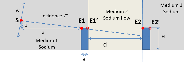
\includegraphics[width=12cm]{ult1.pdf}}
            \slantedcaption{Ultrasonic thermometry configuration used in our study.}
            \label{fig:ult1}
        \end{figure}


    \subsection{Numerical simulations} \label{ssec:2dgrf_num}

        \underline{\textbf{Modeling of the propagation medium}}

            We consider the framework of an effective medium to model the propagation medium. Density and wave velocity of the background model are modified to
incorporate the effects of a heterogeneous medium due to the sodium flow, which only implies temperature gradients.
As mentioned by \cite{Godin2002Aneffectivequiescent},
three conditions have to be met to validate the first hypothesis, which is that of linear behavior, as well as the second hypothesis,
which is that of plane (or quasi-plane) wave propagation. These conditions are that:
\vspace*{-4mm}
            \begin{itemize}
                \item the deviation of the beam must remain weak,
                \item the gradient of the flow velocity relative to the Mach number must remain moderate,
                \item the typical size of the heterogeneities must be large compared to the acoustic wavelength.
            \end{itemize}
\vspace*{-4mm}
            These three conditions were verified and shown to apply in the cases under study in another study based on a ray-tracing code
\parencite{Massacret2014Modellingofultrasonic} and on the analysis of real thermal-hydraulic data \parencite{Tenchine2010Somethermalhydraulic}. Characteristic
sizes of flow heterogeneities, typically ranging between 0.1 cm and 10.0 cm, are also large compared to the wavelengths of the ultrasonic waves considered
\parencite{Grewal1982Watersimulationof}.

            As the measurement area is located just above the outlet of the fuel assembly, the flow is relatively regular and with smooth variations only and
high Reynolds number. In such a case ultrasonic wave propagation is mainly affected by temperature distribution in the flow, and in our study we can therefore
neglect the effects of the speed of the flow. The assumption of an effective medium is thus valid and the propagation medium can then simply be described by
its density and the bulk modulus of the fluid, without having to explicitly model the fluid flow.

            The study of the PLAJEST experiment of mixing cold and hot sodium flows \parencite{Kimura2007Experimentalinvestigationon}, and its detailed
numerical simulation at the French Atomic Commission using the TrioU code \parencite{Brillant2004Largeeddysimulation} leads us to choose a continuous parabolic
variation of temperature inside the jet. Regarding the possible presence of micro-bubbles, there are not enough data for future reactors to currently be able
to take this parameter into account. Doing so will require a complete study, as the influence of the presence of such micro-bubbles will depend on bubble sizes
as well as on transducer frequency \parencite{Cavaro2011Microbubblecloudcharacterization}. The relation between ultrasonic velocity and temperature is given by
equation \ref{eq:3_1}, and equation \ref{eq:3_2} gives the density of sodium as a function of temperature T in Kelvin.

            In order to perform our spectral-element simulations, we first create a mesh of the structure under study using the 'Gmsh' mesh creation tool
\parencite{Geuzaine2009Gmsh:A3}. The mesh created is entirely composed of quadrangles, as required by the spectral-element technique. Around the region of
interest we resort to an absorbing boundary layer called the Perfectly Matched Layer (PML, \cite{Komatitsch2008Anunsplitconvolutional}) in order to efficiently
absorb the outgoing wave field; we use three layers of spectral elements on the outer edges of the mesh in order to implement it. The computational domain has
a size of 723 mm (width) by 156 mm (height) and contains 448,704 elements. We use a polynomial degree N = 4 to define the basis functions in the
spectral-element method, thus each spectral element contains (N + 1)2 = 25 grid points and the total number of unique grid points is 7,108,112. Considering the
sound velocity in liquid sodium at 450\textdegree{}C (2339 m/s) and a dominant frequency of the ultrasonic source of 1 MHz, the number of grid points per
shortest wavelength in the medium is thus approximately 4.7. We simulate a total physical time of 202.5 $\mu$s using a time discretization step of $7.5 \times
10^{-9} \text{s}$, i.e., a total of 27,000 time steps.

            To speed up the calculations we resort to parallel computing on a cluster of computers \parencite{Peter2011Forwardandadjoint}. Once the mesh is
created we thus partition it according to the number of processor cores to be used for the calculation. Each processor core then carries out the calculations
in a sub-domain, and the results are recombined at the end of each time step of the time-stepping algorithm. We perform our calculations using 128 processor
cores.

        \underline{\textbf{Geometry of the assemblies and source description}}

            We select the location to use for the ultrasonic source (S) based on the position of point E1 and on distances a and b in Figure \ref{fig:ult1}.
Values of a and b equal to 100 mm and 12 mm lead to an incidence angle of 7\textdegree{}. To simulate the behavior of the transducer and create a quasi-plane
wave of finite extension we sum 1000 point sources using a Hamming apodization function over a total width of about 67.6 mm. Each point source has a Ricker
(i.e., the second derivative of a Gaussian) wavelet time function with a dominant frequency of 1 MHz \parencite{Cristini2012Someillustrativeexamples}. The
height of the upper part of the stainless steel tube is 50 mm, its thickness is 13 mm and its inner diameter is 100~mm.
            The ratio between the known propagation distance and the time-of-flight difference between echoes E2 and E1 enables us to estimate the velocity of
sound and then, based on equation \ref{eq:3_1}, the mean temperature of the sodium flow on the outer edge of the tube.

        \underline{\textbf{Temperature variations studied}}

            As stated above the propagation medium is in a turbulent state and its temperature distribution varies in a complicated fashion both in space and
in time between, inside and above the assembly edges. \textcite{Buffet1984Studyoftemperature}, \textcite{Fiorina1998Applicationofthe} and
\textcite{Lue2012Stochasticsimulationof} have studied wave propagation in a turbulent liquid metal flow and, regarding sound velocity in such a medium, have
decomposed the medium into two parts: a heterogeneous static part, and a random fluctuation part caused by the turbulent flow.
            In our study we will first perform simulations in the presence of a static temperature distribution only, and then in a second step with
temperature fluctuations in the whole propagation region, generated based on a Gaussian random field.
            \begin{figure}[htbp]
                    \centerline{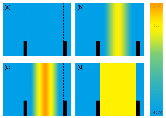
\includegraphics[width=12cm]{ult2.pdf}}
                \slantedcaption{The four types of static temperature fields that we will use in our study: (a) T450, (b) TVAR, (c) TVAR+5, (d) T500. They
differ only between the two edges of the outlet (vertical dotted lines). Model T450 has a constant temperature of 450\textdegree{}C everywhere, TVAR has a
parabolic variation from 450\textdegree{}C to 500\textdegree{}C between the two assembly edges, TVAR+5 has a parabolic variation from 450\textdegree{}C to
505\textdegree{}C, and T500 has a constant temperature of 500\textdegree{}C between the two edges and of 450\textdegree{}C outside.}
                \label{fig:ult2}
            \end{figure}

            \underline{\textbf{Static temperature fields}}

                As shown in Figure \ref{fig:ult2} we select four simple static temperature distributions in and at the outlet of the tube (called "medium 2" in
the following) as well as in the surrounding sodium (called "medium 1"). In the first temperature profile (T450) we consider a homogeneous medium with a
constant temperature of 450\textdegree{}C in both medium 1 and medium 2. It will be our reference case. In the second profile (TVAR) we consider a gradual
evolution of temperature in medium 2, using a symmetric parabolic profile varying from 450\textdegree{}C to 500\textdegree{}C between the edge and the axis of
the tube. Medium 1 still has a constant temperature of 450\textdegree{}C. In the third profile (TVAR+5) we use the same kind of profile as in the second but
with an increase of 5\textdegree{}C, i.e., about \SI{1}{\percent}, of the maximum temperature in medium 2 only. The parabolic profile thus varies from
450\textdegree{}C to 505\textdegree{}C. In the fourth profile (T500) we finally consider a simplified temperature model of 500\textdegree{}C everywhere in the
tube and at its outlet (medium 2) and 450\textdegree{}C everywhere in medium 1.
                In these four media the arrival time of the first echo does not vary, since medium 1 is unchanged. We thus focus our analysis on the variations
of the second echo (wave reflection at point E2 in Figure \ref{fig:ult1}).

            \underline{\textbf{Temperature fluctuation using a Gaussian random field}}

                Gaussian random fields have been developed for digital simulation of multivariate, multidimensional, or multivariate-multidimensional random
processes. They are used for instance in numerical analysis of nonlinear structures, numerical solution of stress wave propagation through a random medium, and
eigenvalue problems of structures that have random homogeneous properties. Here we create Gaussian random fields for the fluctuation of the temperature field
given by,
                \begin{align}\label{eq:3_4}
                    \frac{1}{T(\bm{r})}=\frac{1}{T_0}(1+\epsilon(\bm{r})),
                \end{align}
                where $T(\bm{r})$ is temperature at the spatial position $\bm{r}$, $T_0$ is given by each of the static temperature profiles defined in Figure
\ref{fig:ult2}, and $\epsilon(\bm{r})$ is the fluctuation part calculated by the Gaussian random field.
                Following work on wave propagation in turbulent media (e.g. \textcite{Lue2012Stochasticsimulationof}) we define the randomness of the
temperature fluctuation as an isotropic homogeneous random field by a series cosine functions, expressing $\epsilon(\bm{r})$ as:
                \begin{align}\label{eq:3_5}
                    \epsilon(\bm{r})=\sqrt{2}\sum_{k=1}^N \{S_{\epsilon}(\omega_k)\Delta \omega_k\}^{1/2}cos(\bm{\omega}_k \cdot \bm{r}+\phi_k),
                \end{align}
                where $k$ is the mode number and $N$ is the total number of modes. $\bm{\omega}_k$ is the wave vector, its angle from a coordinate axis of the
wave vector of each mode is $\theta_k = cos^{-1} \frac{\bm{\omega}_k}{|\bm{\omega}_k|}$, and its modulus $|\bm{\omega}_k|=\omega_k$ is defined by
$\omega_k=\omega_l + (k-1)\Delta \omega_k$, linearly distributing it in the range $[\omega_l,\omega_u]$. $\Delta \omega_k = \frac{\omega_u-\omega_l}{N-1}$ is
the wave vector increment. For this process two random input values $\theta_k$ and $\phi_k$ are necessary: $\theta_k$ is distributed uniformly and randomly in
$0\leq\theta_k<2\pi$. Hence its probability density function $Pr$ from 0 to $2\pi$ is $Pr[0\leq\theta_k<2\pi]=1/2\pi$. The other random variety $\phi_k$ is
also uniformly distributed in $0\leq\phi_k\leq 2\pi$. $S_{\epsilon}(\omega_k)$ is the spectral density function and is calculated based on the autocorrelation
function $C_{\epsilon}(r)$ as:
                \begin{align}\label{eq:3_6}
                    S_{\epsilon}(\omega_k)=\frac{1}{2\pi}\int_{-\infty}^\infty C_{\epsilon}(r)e^{-i\omega_kr}dr,
                \end{align}
                where $r$ is the magnitude of the position vector $\bm{r}$ (i.e. $r = |\bm{r}|$). For a Gaussian random field, the autocorrelation function is
defined by a Gaussian distribution following the central limit theorem:
                \begin{align}\label{eq:3_7}
                    C_{\epsilon}(r)=\sigma_{\epsilon}^2R(r)=\sigma_{\epsilon}^2e^{-(r^2/l_{\epsilon}^2)},
                \end{align}
                with $C_{\epsilon}(r)$ the covariance, $R(r)$ the autocorrelation function, $\sigma_{\epsilon}^2$ the variance of the random value, and
$l_{\epsilon}$ the characteristic length of the random pattern. $R$ is the distance between two different points $(\bm{r}_1,\bm{r}_2)$ in the region in which
the random field is simulated, i.e., $r=|\bm{r}_1-\bm{r}_2|$.

                After applying a Fourier transform to equation \ref{eq:3_6} the spectral density function then writes:
                \begin{align}\label{eq:3_8}
                    S_{\epsilon}(\omega_k)=\frac{\sigma_{\epsilon}^2}{2\pi}\int_{-\infty}^\infty e^{-(r^2/l_{\epsilon}^2)}
e^{-i\omega_kr}dr=\frac{\sigma_{\epsilon}^2l_{\epsilon} }{2\sqrt{\pi}}e^{-(\omega_k^2 l_{\epsilon}^2/4)}.
                \end{align}
                We use typical values from the NAJECO experiment \parencite{Tenchine2010Somethermalhydraulic} to choose the characteristic length $l_{\epsilon}
=$ 0.03 m. We set the standard deviation of the fluctuation to $\sigma_\epsilon =$ 0.029 to be able to generate a maximum difference of about 30 degrees
(Figure \ref{fig:ult3}), following a thermal-hydrodynamic calculation result obtained at the French Atomic Commission
\parencite{Tenchine2010Somethermalhydraulic}. The total number of modes $N$ and the range of the wave vector modulus $[\omega_l,\omega_u]$ need to be chosen
carefully: $N$ needs to be large enough to keep a sufficient data set because Equation \ref{eq:3_5} is asymptotically an exact expression for the covariance
function when $N$ tends to infinity \parencite{Shinozuka1972Digitalsimulationof}, and not doing so may introduce numerical errors
\parencite{Mantoglou1982TheTurningBands}. The range $[\omega_l,\omega_u]$ needs to be wide enough to express the entire curve of the spectral density function.
After numerical tests and following a discussion about the minimum requirements of these values in \textcite{Lee2009Effectsoftopography} we select $N$ = 64,
$\omega_u = 6/l_\epsilon$, and $\omega_j=-\omega_u$. (The range of the wave vector needs to be symmetric because the spectral density function of the Gaussian
process is symmetric).

                \begin{figure}[htbp]
                        \centerline{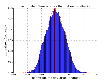
\includegraphics[width=9cm]{ult3.pdf}}
                    \slantedcaption{Distribution of the 30 different temperature fluctuation fields. The magnitude of the fluctuation is defined as the
difference with the average temperature calculated from all fluctuation fields (450\textdegree{}C).}
                    \label{fig:ult3}
                \end{figure}

                \begin{figure}[htbp]
                        \centerline{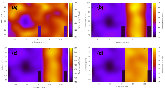
\includegraphics[width=13cm]{ult4.pdf}}
                    \slantedcaption{Examples of generated fluctuating temperature fields obtained when using the (a) T450, (b) TVAR, (c) TVAR+5 and (d) T500
temperature profiles of Figure \ref{fig:ult2}.}
                    \label{fig:ult4}
                \end{figure}

                We generate 30 different patterns of the fluctuation field, and thus obtain 30 temperature fields to be simulated by superimposing the
fluctuation field with the static temperature field based on Equation~\ref{eq:3_4}.
                Figure \ref{fig:ult3} shows the distribution of the magnitude, defined as the difference with the average temperature (450\textdegree{}C), of
the temperature fluctuation for all 30 fluctuation patterns.
                Figure \ref{fig:ult4} shows examples of such generated temperature fields. In the generation of the fluctuation field the origin point of
$\bm{r}$ (i.e., the coordinate of point $\bm{r_1}$) in Equation \ref{eq:3_4} is set at the upper-left corner of the nearest assembly edge. In Figure
\ref{fig:ult4}a the temperature scale is truncated to show the random patterns more clearly. The temperature changes in the vertical shapes along the sodium
jet are due to the temperature profile (see Figure \ref{fig:ult2}); they are right edges in the case of the rectangular profile (Figure \ref{fig:ult4}d) and
more variable edges in the case of a parabolic distribution (Figure \ref{fig:ult4}b and \ref{fig:ult4}c).

                We then carried out simulations of wave propagation in these models and calculated times of flight in the 120 resulting patterns of the
temperature field, constructed by overlaying the 30 Gaussian random field patterns with each of the four types of static temperature profile, as we will
describe in the next section.

    \subsection{Results and discussion} \label{ssec:2dgrf_res}

        \underline{\textbf{Results with static temperature fields}}

            In Figure 5 we show the pressure of the acoustic wave in the computational domain normalized between -1 (blue) and +1 (red), with color intensity
obeying a power law with exponent 0.3 in order to significantly enhance small values for visualization purposes. Such a nonlinear color scale amplifies the
real amplitude of the minor echoes such as the second diffraction E1' in order to observe them more easily. All amplitudes below \SI{1}{\percent} are discarded
in order to avoid visually amplifying very small-amplitude numerical noise. Figure \ref{fig:ult5} highlights several aspects of wave propagation near the upper
part of the fuel assembly. The waves diffracted from edges E1 and E1' are both clearly observed.
            The time $t =$ 88.125 \si{\micro\second} at which the figure is drawn allows us to observe the wave just before it interacts with the second point
E2. Since the incidence angle is very small, the lower part of the wave front goes through the thickness of the tube with a much greater velocity (about 5.8
\si{\milli\meter\per\micro\second} in steel versus about 2.3 \si{\milli\meter\per\micro\second} in sodium) and is well seen as a small wave that propagates
before the main one. Figure \ref{fig:ult5} also shows a superimposition of waves: the main wave and the wave diffracted from E1'. This illustrates the interest
of such snapshots as well as movies of wave propagation in the time domain to facilitate signal analysis and identification of wave fronts in such applications.

            \begin{figure}[htbp]
                    \centerline{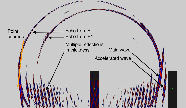
\includegraphics[width=13cm]{ult5.pdf}}
                \slantedcaption{Snapshot of wave propagation at time $t =$ \SI{88.125}{\micro\second} simulated using our spectral-element numerical modeling
technique; we display the pressure variation field (blue being negative and red positive).}
                \label{fig:ult5}
            \end{figure}
%
            Figure \ref{fig:ult6} shows the signals recorded at point S of Figure \ref{fig:ult1} for a time window that allows us to observe the signal
reflected off the second edge (point E2) for the four different temperature configurations. These signals are recorded when the waves come back to the source,
i.e. in the so-called echo mode in non-destructive testing. As wave velocity decreases when sodium temperature increases (Equation \ref{eq:3_1}), the signal is
delayed when temperature increases. The respective time delays of the four signals are qualitatively in agreement with the expected behavior: the hotter medium
2 is, the larger the delay for the time-of-flight from point E2 is as well. We observe a small time difference when the parabolic temperature distribution is
increased by 5\textdegree{}, i.e., by about one percent. The small accelerated wave observed in Figure \ref{fig:ult5} leads to a weaker signal that arrives
before the main echo around time $t =$ \SI{179}{\micro\second}. This signal is \SI{20}{\decibel} lower than the maximum signal because this part of the beam
underwent transmission through steel; in practice in a real experimental setup it could thus be masked by signal noise. Both of these signals are due to the
waves diffracted off point E2. As the duration of the wave corresponds to about two periods, similar to a highly damped transducer, no interferences occur
between these two waves; this can also be seen in Figure \ref{fig:ult5}, in which the waves are clearly separated.

            In order to perform a more quantitative analysis, in Table \ref{table:ult1} we give the arrival times in \si{\micro\second} of the second echo
measured at the signal maximum. Corresponding pressures have arbitrary units because, since the wave equation is linear, the amplitudes of the signals do not
significantly vary and thus amplitude cannot be used to detect temperature variations in this configuration; we thus analyze arrival times only in our study.
            The changes in the time-of-flight of the second echo at point E2 provide information on the ability and sensitivity of the method to detect small
temperature variations in the case of the absence of temperature fluctuation. Between Simulations 2 and 3 we find that the increase of 5\textdegree{}C of the
maximum of the temperature profile leads to a shift of \SI{68}{\nano\second}. As the time of flight of echo E1 is always the same, this difference is also the
difference between the times of flight of the echoes on the two edges ($t_{E2} - t_{E1}$). In a reactor such a time difference could be measured using a
\SI{1}{\mega\hertz} signal, i.e., a short signal, but that would require good signal-to-noise ratio and signal stability.

            \begin{figure}[htbp]
                    \centerline{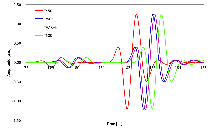
\includegraphics[width=16cm]{ult6.pdf}}
                \slantedcaption{Comparison between the echoes reflected off point E2 in the four simulations performed for the model with right-angle edges.}
                \label{fig:ult6}
            \end{figure}

            \begin{table}
                \centering
                \slantedcaption{Time-of-flight and amplitude of the echo coming back from point E2 for the four different temperature configurations in the
case of a right-angle geometry.}
\vspace{5truemm}
                \begin{tabular}{lll}
                Configuration    & \parbox[t]{5cm}{Arrival time of\\the second echo (\si{\micro\second}) $t_{E2}$} & \parbox[t]{5cm}{Maximum amplitude \\
(arbitrary units)} \\ \hline
                1. T450          & \num{182.346}                  & \num{1.24284}                   \\
                2. TVAR          & \num{183.000}                  & \num{1.24971}                   \\
                3. TVAR+5        & \num{183.068}                  & \num{1.25112}                   \\
                4. T500          & \num{183.330}                  & \num{1.24801}                   \\
                \end{tabular}
                \label{table:ult1}
            \end{table}


        \textit{\textbf{Results with temperature fluctuation}}

            \underline{\textbf{Effect of temperature fluctuation on time-of-flight}}

                Let us now study the fluctuation in times of flight when temperature fluctuations in the medium are taken into account and see if it is still
possible to detect such short time differences. We simulate wave propagation for \num{30} random temperature fields added to each of the four static fields,
leading to a total of \num{120} different propagation media, and obtain fluctuations of the time of flight for echo E2 but also for echo E1. We thus consider
that the fluctuating media introduce a random noise around the true time of flight corresponding to a static situation. Figure \ref{fig:ult7} shows the
resulting distribution of time of flight $t_{E2}$ for the four static temperature cases. We observe an overlapping of various times of flight. An averaging
procedure would be necessary to reconstruct the true time of flight as defined above. Table \ref{table:ult2} summarizes time of flight measurements for both
the E1 and E2 echoes without fluctuations (left column) and using averaged times of flight in the case of stochastic fluctuations (right column). We then
calculate the time difference between the two echoes ($t_{E2} - t_{E1}$), as this variation of the time difference would be a signature of variation in the
sodium jet. The \num{5}\textdegree{}C difference between the two parabolic profiles TVAR and TVAR+5 creates a \SI{68}{\nano\second} difference between the
times of flight difference from edges E2 and E1. This time difference is equal to about \SI{66}{\nano\second} when an average process is performed over
\num{30} fluctuating temperature field.

                \begin{figure}[htbp]
                        \centerline{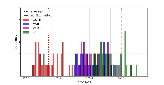
\includegraphics[width=20.5cm]{ult7.pdf}}
                    \slantedcaption{Distributions of variation of times of flight resulting from temperature fluctuations for each of the \num{120}
temperatures profiles considered, i.e. the \num{30} random profiles superimposed to each of the four static temperature profiles.}
                    \label{fig:ult7}
                \end{figure}

                \begin{table}
                    \small
                    \centering
                    \slantedcaption{Variations of time of flight between results for the cases without temperature fluctuations and averaged results from
\num{30} measurements in cases with fluctuations.}
\vspace{5truemm}
                    \begin{tabular}{lll} \hline
                                  & $t_{E2}$ without fluctuation (\si{\micro\second}) & \parbox[t]{5cm}{Averaged $t_{E2}$ from \num{30}\\measurements
(\si{\micro\second})} \\ \hline
                    T450          & \num{182.346}                  & \num{182.354}                   \\
                    TVAR          & \num{183.000}                  & \num{183.008}                   \\
                    TVAR+5        & \num{183.068}                  & \num{183.074}                   \\
                    T500          & \num{183.330}                  & \num{183.337}                   \\
                                  & $t_{E1}$ without fluctuation (\si{\micro\second}) & \parbox[t]{5cm}{Averaged $t_{E1}$ from \num{30}\\measurements
(\si{\micro\second})} \\ \cline{2-3}
                    T450          & \num{86.250}                  & \num{86.266}                   \\
                    TVAR          & \num{86.250}                  & \num{86.266}                   \\
                    TVAR+5        & \num{86.250}                  & \num{86.266}                   \\
                    T500          & \num{86.250}                  & \num{86.266}                   \\
                                  & \parbox[t]{5cm}{Time difference ($t_{E2}-t_{E1}$) without fluctuation (\si{\micro\second})} & \parbox[t]{5cm}{Time
difference\\($t_{E2}-t_{E1}$) averaged $t_{E2}$ from\\\num{30} measurements (\si{\micro\second})} \\ \cline{2-3}
                    T450          & \num{96.098}                  & \num{96.088}                   \\
                    TVAR          & \num{96.750}                  & \num{96.742}                   \\
                    TVAR+5        & \num{96.818}                  & \num{96.808}                   \\
                    T500          & \num{97.080}                  & \num{97.071}                   \\
                                  & \parbox[t]{5cm}{Variation of time difference\\$\Delta(t_{E2}-t_{E1})$ between TVAR and TVAR+5 without\\fluctuation
(\si{\micro\second})} & \parbox[t]{5cm}{Variation of time difference\\$\Delta(t_{E2}-t_{E1})$ between TVAR\\and TVAR+5 averaged from\\\num{30} measurements
(\si{\micro\second})} \\ \cline{2-3}
                    $(t_{E2}-t_{E1})_{TVAR}$          & \num{10.500}                  & \num{10.476}                   \\
                    $(t_{E2}-t_{E1})_{TVAR+5}$        & \num{10.568}                  & \num{10.542}                   \\
                    \parbox[t]{5cm}{$\Delta(t_{E2}-t_{E1})=$\\$(t_{E2}-t_{E1})_{TVAR+5}\\-(t_{E2}-t_{E1})_{TVAR}$}       & \SI{68}{\nano\second}
  & \SI{66}{\nano\second}                   \\\hline
                    \end{tabular}
                    \label{table:ult2}
                \end{table}

            \underline{\textbf{Detection of variations of statistic temperature by averaging}}

                In Figure \ref{fig:ult8} we perform a more complete statistical analysis. If we calculate the standard deviation of time-of-flight measurements
due to the random pattern in the temperature fields we can evaluate the probability of success to separate times of flight for a \SI{1}{\percent} temperature
difference, i.e., 5\textdegree{}C in our case.

In Table \ref{table:ult2} we find that the variation in the time-of-flight difference $\Delta(t_{E2}-t_{E1})$
between echoes E2 and E1 due to the \SI{1}{\percent} temperature difference is \SI{68}{\nano\second} in the case of static temperature fields; Considering
classical Gaussian statistics, it is possible to statistically separate the two time-of-flights differences $\Delta(t_{E2}-t_{E1})$ with a
\SI{68}{\percent} chance of success if the standard deviation of the time-of-flight measurements is lower than \SI{34}{\nano\second} (\num{2}$\sigma$).
To improve the chance of success the standard deviation should be lower than \SI{17}{\nano\second} (\num{4}$\sigma$) to separate times of flight with
\SI{95}{\percent} of success, and lower than \SI{11}{\nano\second} (\num{6}$\sigma$) to separate times of flight with \SIlist{99}{\percent} of
success. Figure \ref{fig:ult8} shows that these levels of confidence are reached when using respectively \num{15}, \num{24} and \num{28} measurements.

                \begin{figure}[htbp]
                        \centerline{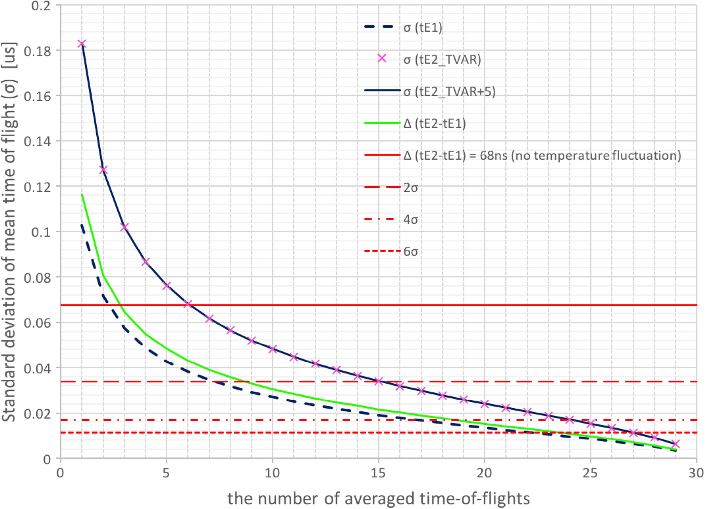
\includegraphics[width=16cm]{ult8.pdf}}
                    \slantedcaption{Variation of the standard deviation of the mean time-of-flight with respect to the number of times-of-flight used to
calculate the mean value.}
                    \label{fig:ult8}
                \end{figure}

\vspace*{-0.8truecm}
\section{Conclusions of this chapter}

In \autoref{sec:UPSILON}, we demonstrated the accuracy and efficiency of the SEM for our application, i.e. application to a heterogeneous medium (silicon oil)
using a \SI{2.25}{\mega\hertz} acoustic wave.
The results calculated with the SEM were compared with several FDTD methods, including a classic 2nd-order FDTD, a 4th-order FDTD,
and two types of more-recently developed methods, namely the optimized FDTD and Non-Standard FDTD.
Even if those recent FDTD methods showed good convergence properties, the SEM exhibited higher numerical efficiency for the problems that we want to study.

In \autoref{sec:2DGRF}, we presented a 2D numerical modeling study based on a spectral-element method in the time domain to analyze variations of time of flight due to
temperature changes in a fluid medium. We have shown that our numerical approach can accurately model the principle of ultrasonic thermometry above the core of
a Sodium Fast Reactor. Based on our numerical approach we have illustrated the sensitivity of an ultrasonic thermometry method to a relatively weak temperature
change. In the simulations with a static temperature profile we have shown that a temperature variation of about \SI{1}{\percent} of the average temperature
could be detected, as this temperature variation induces a time shift of about \SI{68}{\nano\second}.

We generated 120 patterns of temperature fields using a Gaussian random field and examined their effect on the time-of-flight of the signal reflected
off the assembly edges. We investigated the effect of temperature fluctuations on the variations of times-of-flight for four different patterns of static
temperature profiles. Under these thermodynamically and acoustically complex conditions we found that it may be difficult to detect a \num{5}-degree i.e. one
percent variation in the static temperature field based on a single measurement, but also showed that by averaging times-of-flight coming from about \num{30}
measurements such detection becomes possible with a high level of confidence.

We took the thermal static heterogeneity of the medium into account by considering a simplified medium and superimposing fluctuations created
based on a random field generator. In the next chapter of this thesis, we will extend our simulations to take into account a more realistic medium defined
using computational fluid dynamics results for new reactor designs that are currently
being performed in a project called ASTRID (Advanced Sodium Technological Reactor for Industrial Demonstration) \parencite{Coz2011Sodiumcooledfast}.
Taking flow rates i.e. a moving fluid into account will require further development of our spectral-element technique in future work. In addition to using a more complete
description of liquid sodium above the fuel assemblies, further studies should also focus on better understanding the origin of signal noise to understand
which part could be produced by medium fluctuations such as eddies or vortices. The results that we have obtained can be useful for ultrasonic thermometry, but
our conclusions should also be valid for telemetry applications in which time-of-flight measurements are used to accurately locate objects in a liquid medium.

The study in this section relied on the hypothesis that the temperature field in the region near the outlet may be described by superimposing a static
field and a fluctuation field. The static field was provided as simple profiles, for instance having a parabolic shape. The fluctuation fields were generated
using a Gaussian random field.
However, at the moment, the Gaussian random field method is only validated for fields without strong flows,
and thus we are still not sure to what extent a Gaussian random field hypothesis is applicable for regions in which flows with strong variations may exist.
It is expected that Gaussian random fields are applicable to simulate regions that are located sufficiently far from the outlets of the sodium flow,
but less applicable in regions located closer to the outlets. Hence, in future studies, it will be necessary to examine the applicability of a Gaussian random field
approximation to represent medium fluctuations, depending on the distance from the sodium outlets, by comparing the results obtained based on wave propagation in a medium
represented by a Gaussian random field to those coming from a computational fluid dynamics (CFD) simulation.

